\section{Introduction}
\begin{sloppypar}
To ensure the quality of software products and to automate the testing and release process, 
Continuous integration and deployment are usually the go to paradigms in modern software engineering.
\begin{figure}[ht]
    \begin{center}
        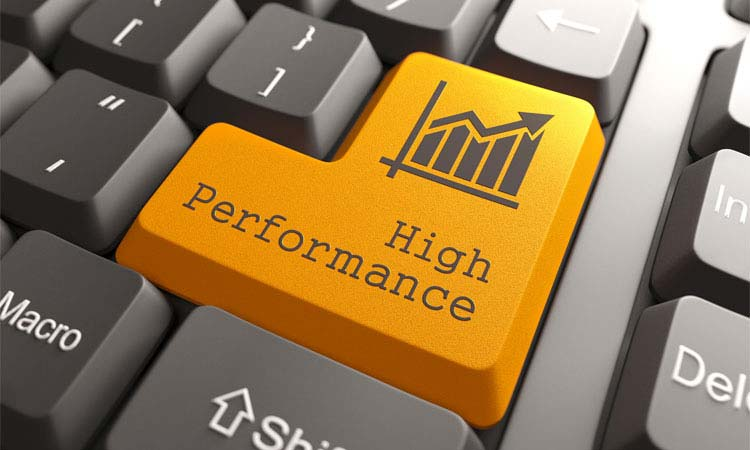
\includegraphics[width=12cm]{./performance.jpg}
    \end{center}
    \setcaptioncitation{https://www.dlr.de/sc/desktopdefault.aspx/tabid-11647/}
    
    \caption{}
\end{figure}

The performance of software is usually mesured through Benchmarks which conain a full set of specifications needed to enable the evaluation of the performance of a certain aspect of the system.
Benchmarks usually contain a scenario, performance evaluation criteria and a benchmarking score. 
\clearpage
\begin{figure}[ht]
    \begin{center}
        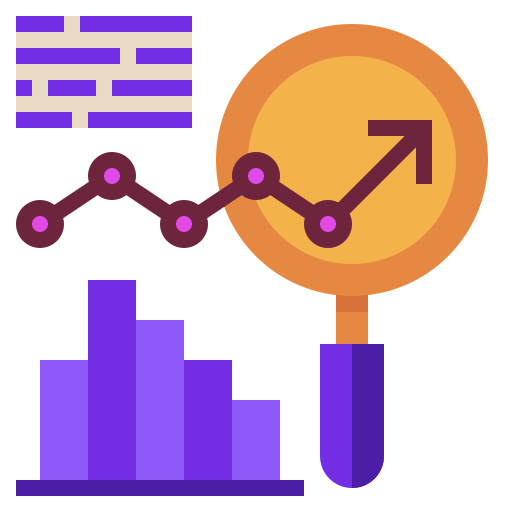
\includegraphics[width=8cm]{./benchmark.png}
    \end{center}
    \setcaptioncitation{https://www.flaticon.com/authors/becris}
    \caption{}
\end{figure}

Using these values not only gives us the ability to understand the performance of the system and also to enable fair comparison between different solutions, 
or between subsequent developments of the system, which help us make sure that new system releases are better or at least as "good" as the previous ones

\begin{figure}[ht]
    \begin{center}
        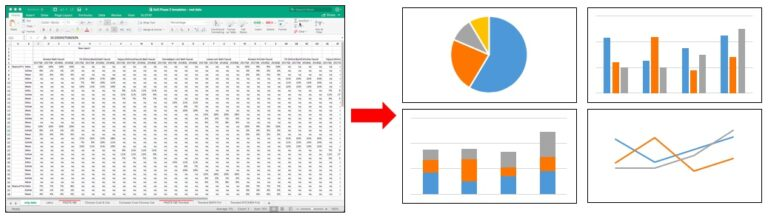
\includegraphics[width=9cm]{./data-to-charts.jpg}
    \end{center}
    \setcaptioncitation{https://www.cpgdatainsights.com/communicate-insights}
    \caption{}
\end{figure}

Since "a picture is worth a thousand words", visualizating the data in a coherant way can help the users get a sense of what's going on and take action.
Generating these visualizations manually can be a tidious task that if not done properly may produce a chart that is hard to read or even misleading.
The purpose of our project is to make the usage of visualizations as easy as possible which help reducing the time needed to analyse the system and taking actions if needed.

\end{sloppypar}
